\documentclass[border=10pt]{standalone}

\usepackage{tikz}
\usepackage{tikzsymbols}
\usetikzlibrary{calc,patterns,shapes.geometric}

\def\centerarc[#1](#2)(#3:#4:#5){\draw[#1] ($(#2)+({#5*cos(#3)},{#5*sin(#3)})$) arc (#3:#4:#5);}

\begin{document}
	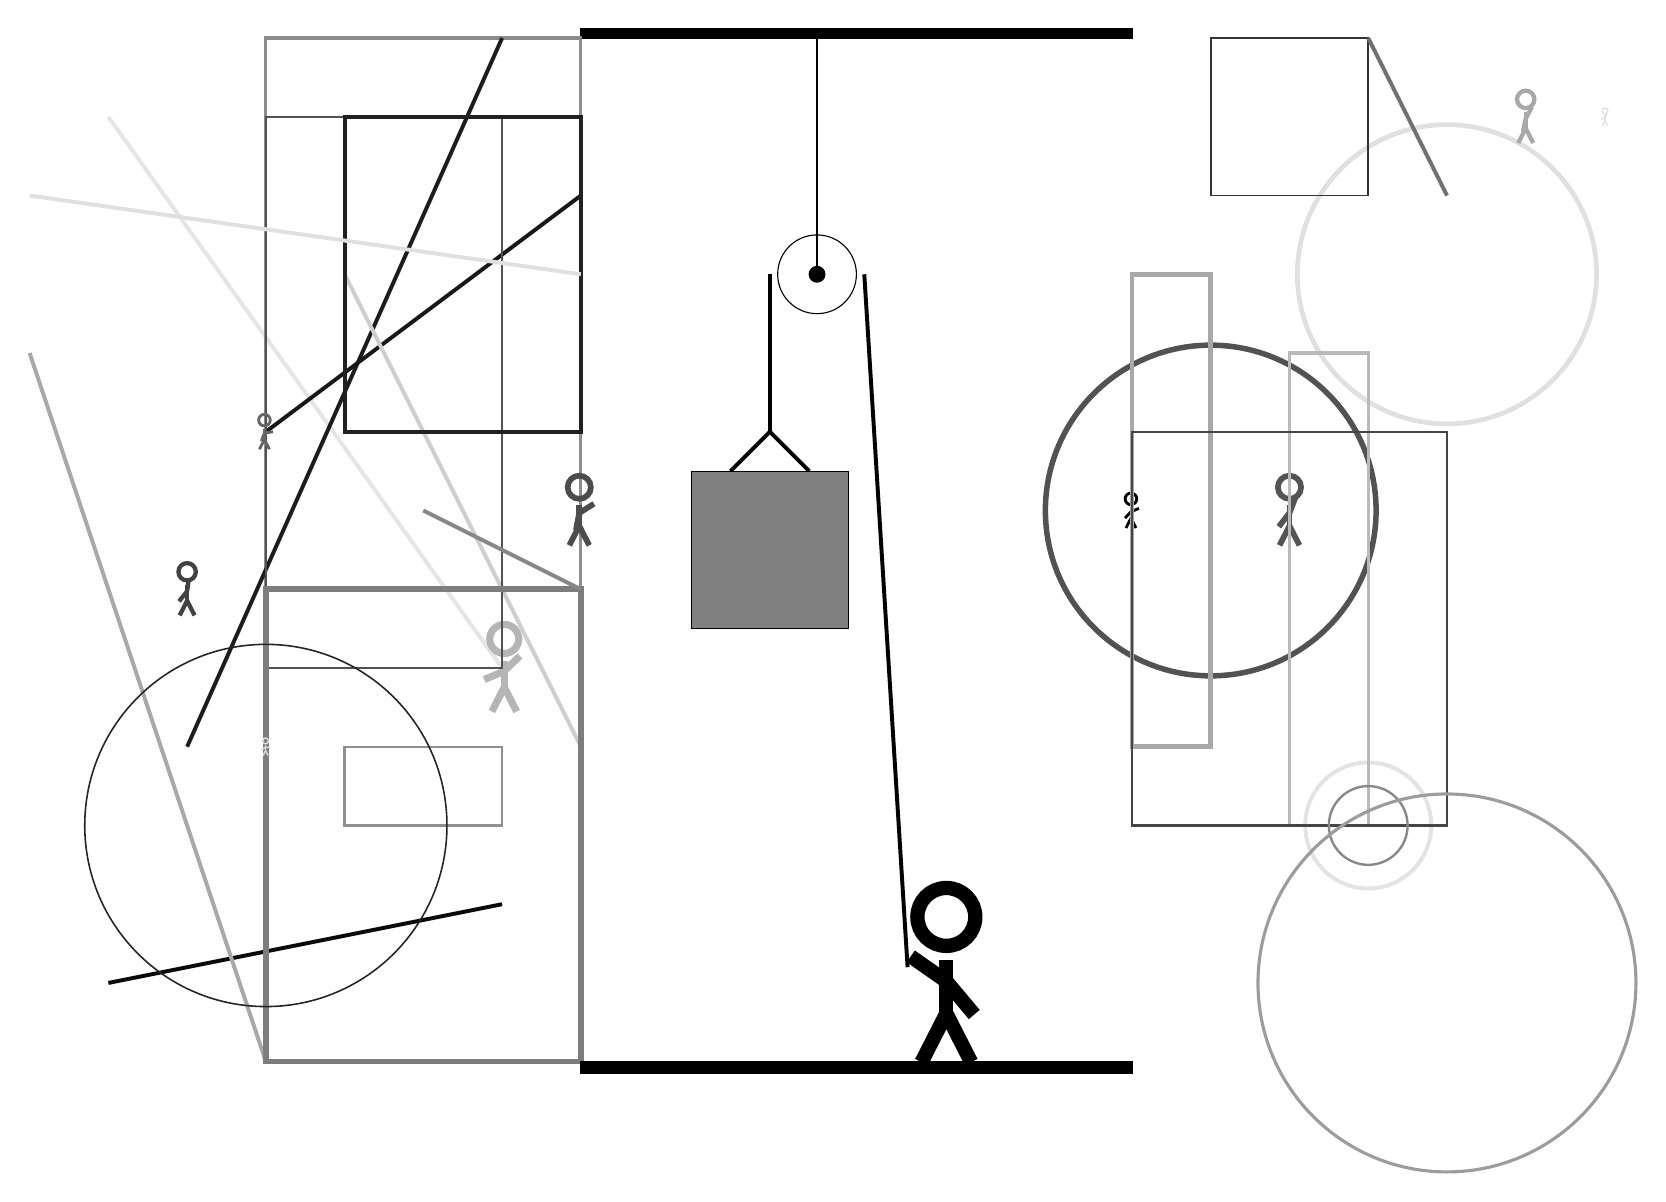
\begin{tikzpicture}
		%%%%% START %%%%%
		
		\draw[fill=black] (-2, 10) rectangle (5, 10.125);
		
		\draw (1, 7) circle (0.5);
		\draw[fill=black] (1, 7) circle (0.1);
		\draw (1, 10) -- (1, 7);
		
		\draw[line width=0.5mm] (-0.1, 4.5) -- (0.4, 5.0) -- (0.9, 4.5);
		\draw[fill=black!50] (-0.6, 4.5) rectangle (1.4, 2.5);
		
		\node[line width=0.3mm, color=black!67] at (7, 4) {\Strichmaxerl[4][52][69]};
		
		\draw[line width=0.5mm, color=black!10](-3, 2) -- (-8, 9);
		\draw [line width=0.7mm, color=black!68](6, 4) circle (2.1);
		\draw[line width=0.5mm, color=black!96](-3, -1) -- (-8, -2);
		\draw[line width=0.4mm, color=black!45] (-2, 10) rectangle (-6, -3);
		\node[line width=0.4mm, color=black!29] at (-3, 2) {\Strichmaxerl[5][23][44]};
		\draw[line width=0.5mm, color=black!89](-7, 1) -- (-3, 10);
		\draw[line width=0.5mm, color=black!91](-2, 8) -- (-6, 5);
		\draw[line width=0.5mm, color=black!19](-2, 1) -- (-5, 7);
		
		\draw[line width=0.5mm, color=black!34](-6, -3) -- (-9, 6);
		
		\draw[line width=0.2mm, color=black!68] (-3, 2) rectangle (-6, 9);
		
		\draw[line width=0.5mm, color=black!87] (-2, 5) rectangle (-5, 9);
		\draw[line width=0.7mm, color=black!51] (-2, 3) rectangle (-6, -3);
		
		\node[line width=0.6mm, color=black!100] at (5, 4) {\Strichmaxerl[2][47][23]};
		\draw [line width=0.6mm, color=black!12](9, 7) circle (1.9);
		\draw[line width=0.3mm, color=black!44] (-3, 1) rectangle (-5, 0);
		
		\draw [line width=0.5mm, color=black!11](8, 0) circle (0.8);
		\draw[line width=0.4mm, color=black!27] (7, 6) rectangle (8, 0);
		\node[line width=0.2mm, color=black!60] at (-6, 5) {\Strichmaxerl[2][69][8]};
		
		\draw[line width=0.5mm, color=black!47](-4, 4) -- (-2, 3);
		\node[line width=0.3mm, color=black!12] at (11, 9) {\Strichmaxerl[1][25][62]};
		\draw[line width=0.6mm, color=black!34] (5, 7) rectangle (6, 1);
		
		\node[line width=0.7mm, color=black!70] at (-2, 4) {\Strichmaxerl[4][79][32]};
		\draw[line width=0.3mm, color=black!73] (5, 0) rectangle (9, 5);
		\node[line width=0.2mm, color=black!34] at (10, 9) {\Strichmaxerl[3][78][62]};
		\draw[line width=0.2mm, color=black!80] (6, 10) rectangle (8, 8);
		\draw [line width=0.2mm, color=black!86](-6, 0) circle (2.3);
		\draw [line width=0.3mm, color=black!47](8, 0) circle (0.5);
		\node[line width=0.5mm, color=black!13] at (-6, 1) {\Strichmaxerl[1][31][3]};
		
		\draw[line width=0.5mm, color=black!12](-2, 7) -- (-9, 8);
		\draw [line width=0.4mm, color=black!39](9, -2) circle (2.4);
		\draw[line width=0.5mm, color=black!56](8, 10) -- (9, 8);
		\node[line width=0.2mm, color=black!74] at (-7, 3) {\Strichmaxerl[3][52][82]};
		
		\draw[line width=0.5mm] (0.4, 7) -- (0.4, 5.0);
		\centerarc[line width=0.5mm](1, 7)(0:180:0.6);
		\draw[line width=0.5mm](1.6, 7) -- (2.15, -1.8);
		
		\node at (2.6, -1.9) {\Strichmaxerl[10][-35][-50]};
		
		\draw[fill=black] (-2, -3) rectangle (5, -3.15);
		
		%%%%% END %%%%%
	\end{tikzpicture}
\end{document}